% This is a Basic Assignment Paper but with like Code and stuff allowed in it, there is also url, hyperlinks from contents included. 

\documentclass[11pt]{article}

% Preamble

\usepackage[margin=1in]{geometry}
\usepackage{amsfonts, amsmath, amssymb}
\usepackage{fancyhdr, float, graphicx}
\usepackage[utf8]{inputenc} % Required for inputting international characters
\usepackage[T1]{fontenc} % Output font encoding for international characters
\usepackage{fouriernc} % Use the New Century Schoolbook font
\usepackage[nottoc, notlot, notlof]{tocbibind}
\usepackage{listings}
\usepackage{xcolor}
\usepackage{blindtext}
\usepackage{hyperref}
\hypersetup{
    colorlinks=true,
    linkcolor=black,
    filecolor=magenta,      
    urlcolor=cyan,
    pdfpagemode=FullScreen,
    }

\definecolor{codegreen}{rgb}{0,0.6,0}
\definecolor{codegray}{rgb}{0.5,0.5,0.5}
\definecolor{codepurple}{rgb}{0.58,0,0.82}
\definecolor{backcolour}{rgb}{0.95,0.95,0.92}

\lstdefinestyle{mystyle}{
    backgroundcolor=\color{backcolour},   
    commentstyle=\color{codegreen},
    keywordstyle=\color{magenta},
    numberstyle=\tiny\color{codegray},
    stringstyle=\color{codepurple},
    basicstyle=\ttfamily\footnotesize,
    breakatwhitespace=false,         
    breaklines=true,                 
    captionpos=b,                    
    keepspaces=true,                 
    numbers=left,                    
    numbersep=5pt,                  
    showspaces=false,                
    showstringspaces=false,
    showtabs=false,                  
    tabsize=2
}

\lstset{style=mystyle}

% Header and Footer
\pagestyle{fancy}
\fancyhead{}
\fancyfoot{}
\fancyhead[L]{\textit{\Large{Information and Cycbersecurity - 2nd Year B. Tech}}}
%\fancyhead[R]{\textit{something}}
\fancyfoot[C]{\thepage}
\renewcommand{\footrulewidth}{1pt}



% Other Doc Editing
% \parindent 0ex
%\renewcommand{\baselinestretch}{1.5}

\begin{document}

\begin{titlepage}
    \centering

    %---------------------------NAMES-------------------------------

    \huge\textsc{
        MIT World Peace University
    }\\

    \vspace{0.75\baselineskip} % space after Uni Name

    \LARGE{
        Information and Cybersecurity\\
        Second Year B. Tech, Semester 1
    }

    \vfill % space after Sub Name

    %--------------------------TITLE-------------------------------

    \rule{\textwidth}{1.6pt}\vspace*{-\baselineskip}\vspace*{2pt}
    \rule{\textwidth}{0.6pt}
    \vspace{0.75\baselineskip} % Whitespace above the title



    \huge{\textsc{
            Learning to Work with NESSUS tool for Vulnerability Assessment
        }} \\



    \vspace{0.5\baselineskip} % Whitespace below the title
    \rule{\textwidth}{0.6pt}\vspace*{-\baselineskip}\vspace*{2.8pt}
    \rule{\textwidth}{1.6pt}

    \vspace{1\baselineskip} % Whitespace after the title block

    %--------------------------SUBTITLE --------------------------	

    \LARGE\textsc{
        Lab Assignment 11
    } % Subtitle or further description
    \vfill

    %--------------------------AUTHOR-------------------------------

    Prepared By
    \vspace{0.5\baselineskip} % Whitespace before the editors

    \Large{
        Krishnaraj Thadesar \\
        Cyber Security and Forensics\\
        Batch A1, PA 20
    }


    \vspace{0.5\baselineskip} % Whitespace below the editor list
    \today

\end{titlepage}


\tableofcontents
\thispagestyle{empty}
\clearpage

\setcounter{page}{1}

\section{Aim}
Configuration and demonstration of NESSUS tool for vulnerability assessment

\section{Objectives}
To learn authentication technique for access control

\section{Theory}
\subsection{Vulnerability Assessment}
Vulnerability assessment is the process of identifying and evaluating potential security vulnerabilities in a computer system or network. This assessment helps organizations to identify and prioritize potential risks and develop strategies to mitigate them. One of the popular vulnerability assessment tools is Nessus.\\

Nessus is a widely used vulnerability assessment tool that is designed to scan and detect vulnerabilities in networks, systems, and applications. Here are some of the features of Nessus:
\begin{enumerate}
    \item Multiple scanning options: Nessus offers various scanning options, including network, web application, and database scanning. It supports multiple protocols, such as TCP/IP, SNMP, SSH, and HTTP/HTTPS.
    \item Comprehensive vulnerability database: Nessus maintains a comprehensive database of known vulnerabilities and exploits, which it uses to identify potential vulnerabilities in the target system.
    \item Customizable policies: Nessus allows users to customize scan policies based on their specific needs. Users can create policies to scan specific IP addresses, ports, or protocols.
    \item Real-time alerts: Nessus provides real-time alerts on critical vulnerabilities, enabling organizations to quickly remediate potential threats.
    \item Compliance reporting: Nessus generates compliance reports based on industry standards such as PCI DSS, HIPAA, and CIS.
    \item Integration with other tools: Nessus can integrate with other security tools such as SIEMs and incident response platforms.

\end{enumerate}

\subsection{How Nessus Works}
\begin{enumerate}
    \item Discovery: Nessus starts by discovering devices on the network, including servers, workstations, routers, and switches.
    \item Scan configuration: The user configures the scan policy based on their needs, such as IP range, scanning ports, protocols, and vulnerabilities to scan for.
    \item Scan execution: Nessus then scans the target system for vulnerabilities based on the configured policy. The scanning process may take some time, depending on the size of the network and the complexity of the scan policy.
    \item Vulnerability assessment: Nessus then analyzes the scan results and reports potential vulnerabilities. It provides detailed information on the type of vulnerability, the level of severity, and possible remediation actions.
    \item Reporting: Nessus generates a report that summarizes the vulnerabilities found during the scan. The report includes detailed information on each vulnerability, including its severity level and recommended remediation actions.
\end{enumerate}

\section{Platform}
\textbf{\textbf{Operating System}}: Arch Linux x86-64 \\
\textbf{\textbf{IDEs or Text Editors Used}}: Visual Studio Code\\
\textbf{\textbf{Compilers or Interpreters} }: Python 3.10.1\\

\section{Input and Output}
\begin{figure}[H]
    \centering
    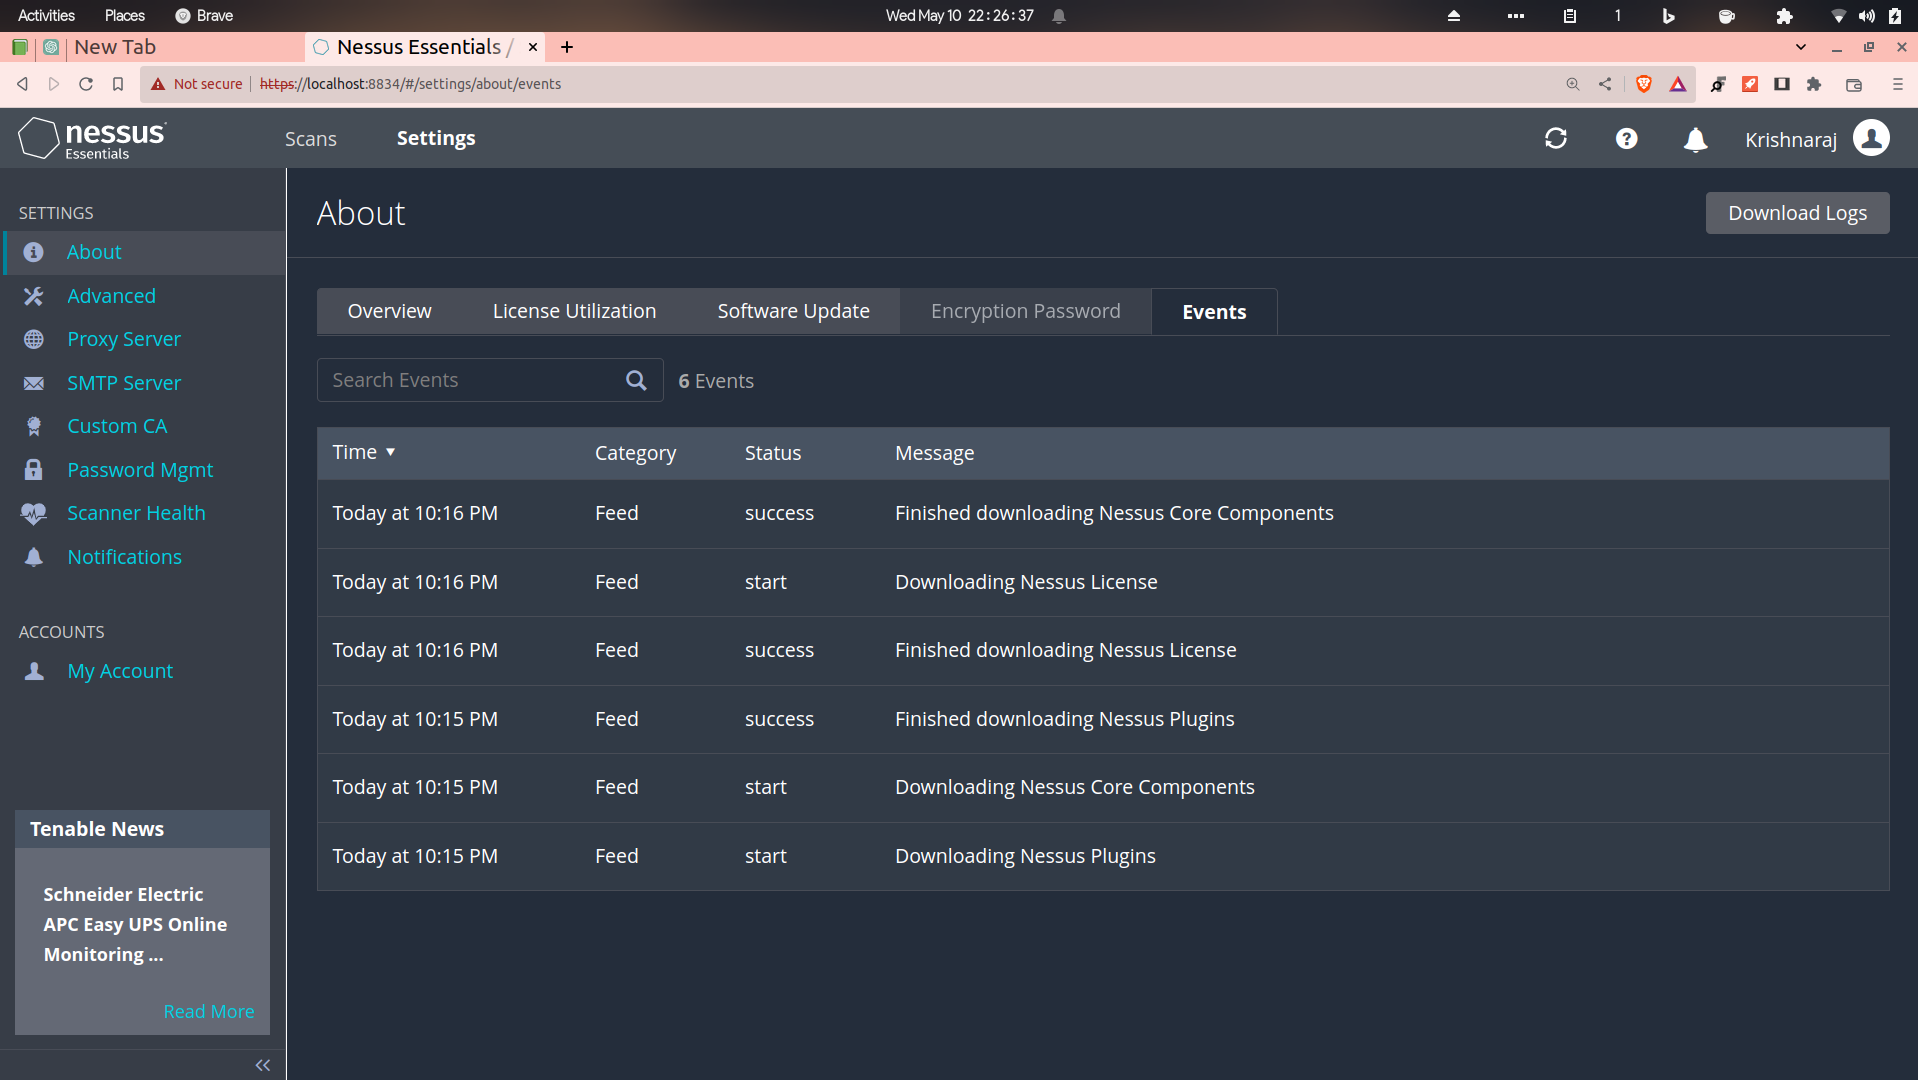
\includegraphics[width=.45\textwidth]{nessus 1.png}
    \caption{Nessus Home Page}
\end{figure}
\begin{figure}[H]
    \centering
    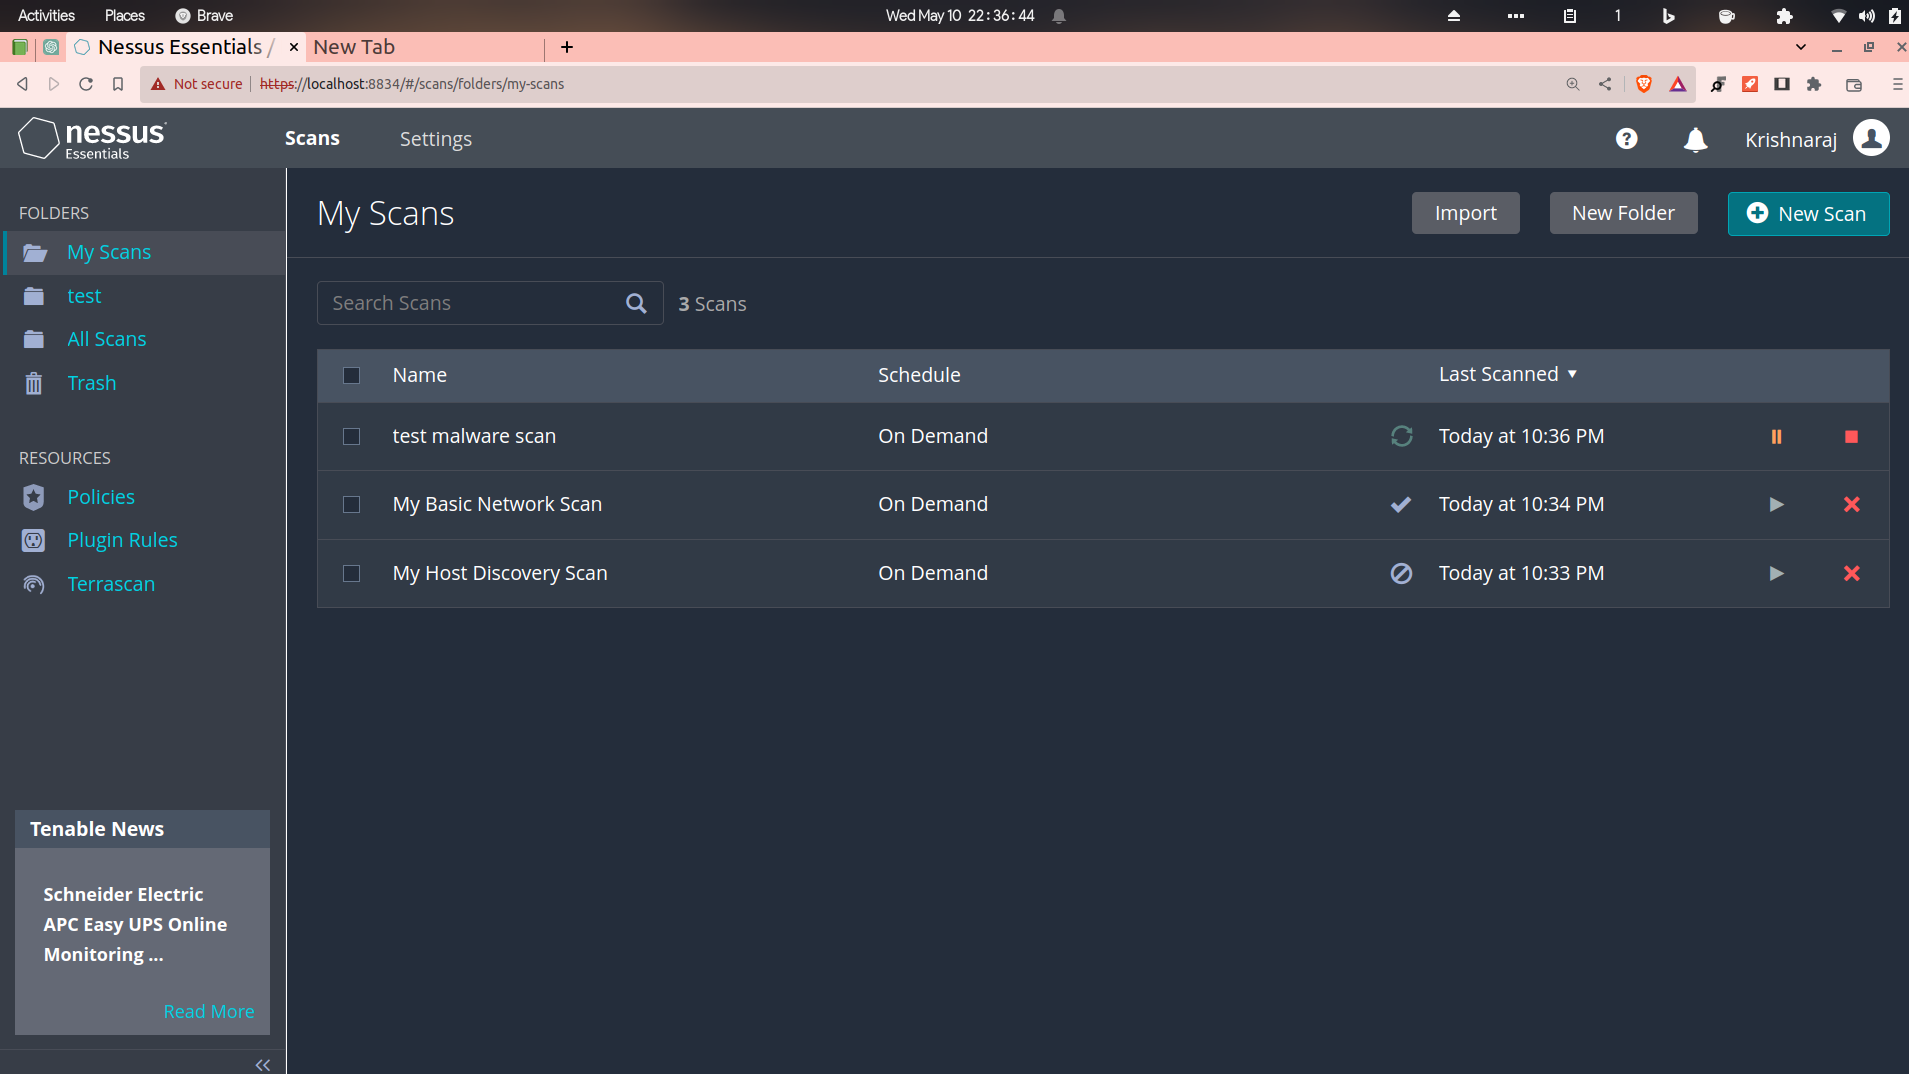
\includegraphics[width=.45\textwidth]{nessus 2.png}
    \caption{Nessus Scans}
\end{figure}
\begin{verbatim}
\end{verbatim}


% \section{Code}
% \lstinputlisting[language=Python, caption="DSA Signature Validity using PyCrypto Library"]{../Programs/Assignment_7/dsa using lib.py}

\section{Conclusion}
Thus, we have learnt about the authentication technique for access control, and implemented it using NESSUS tool for vulnerability assessment.Thus, we have seen how to implement digital signatures using DSA algorithm.
\clearpage

\section{FAQ}

\begin{enumerate}

    \item \textbf{What vulnerabilities can Nessus detect?}\\

          Nessus is a vulnerability scanner that can detect a wide range of vulnerabilities in an IT environment, including:

          \begin{enumerate}
              \item Operating system vulnerabilities: Nessus can identify vulnerabilities in the operating systems of network devices, servers, and workstations, including Windows, Linux, Unix, and macOS.
              \item Application vulnerabilities: Nessus can detect vulnerabilities in popular applications such as web browsers, email clients, and office productivity software.
              \item Network vulnerabilities: Nessus can identify network vulnerabilities, including weak passwords, open ports, and misconfigured network devices.
              \item Malware and botnets: Nessus can detect signs of malware and botnets on network devices and workstations.
              \item Web application vulnerabilities: Nessus can identify vulnerabilities in web applications, including SQL injection, cross-site scripting, and directory traversal.
          \end{enumerate}
    \item \textbf{What are the limitations of Nessus essentials?}\\

          Nessus Essentials is a free version of the Nessus vulnerability scanner that is limited in its capabilities compared to the paid version. Some of the limitations of Nessus Essentials include:

          \begin{itemize}
              \item Limited scanning: Nessus Essentials is limited to scanning up to 16 IP addresses or hosts at a time, while the paid version can scan thousands of hosts.
              \item No scheduling: Nessus Essentials does not allow users to schedule scans or automated reporting, which can be inconvenient for organizations with large IT environments.
              \item Limited vulnerability coverage: Nessus Essentials has a smaller set of plugins for detecting vulnerabilities compared to the paid version, which can limit its effectiveness in identifying security issues.
              \item No support: Nessus Essentials does not come with technical support from Tenable, the company behind Nessus.
          \end{itemize}
    \item \textbf{How can you identify a false positive vulnerability in Nessus?}\\

          A false positive vulnerability in Nessus occurs when the scanner reports a vulnerability that does not actually exist. To identify false positive vulnerabilities in Nessus, follow these steps:

          \begin{itemize}
              \item Verify the vulnerability: Check the affected device or application to verify if the reported vulnerability actually exists.
              \item Check the plugin output: Review the Nessus plugin output to identify any discrepancies or errors that may have led to the false positive.
              \item Confirm with multiple sources: Check other vulnerability scanners, security advisories, and technical forums to confirm if the vulnerability is a known issue.
              \item Perform additional testing: Conduct additional testing or penetration testing to confirm if the vulnerability can be exploited.
          \end{itemize}

    \item \textbf{How many hosts can Nessus scan? What port does Nessus use?}\\

          The number of hosts that Nessus can scan depends on the version of the software and the license purchased. The free version of Nessus, Nessus Essentials, can scan up to 16 IP addresses or hosts at a time, while the paid versions can scan thousands of hosts.\\

          Nessus uses various ports to communicate with the devices being scanned. The default port used by Nessus is 8834 for web-based communication, but Nessus can also use other ports depending on the type of scan being performed. For example, Nessus may use port 22 for SSH communication or port 445 for SMB communication.
\end{enumerate}

\end{document}